\documentclass[a4paper,12pt]{report}

\usepackage{alltt, fancyvrb, url}
\usepackage{graphicx}
\usepackage[utf8]{inputenc}
\usepackage{float}
\usepackage{hyperref}

\hypersetup{
    colorlinks=true,
    linkcolor=black,
    filecolor=magenta,      
    urlcolor=blue,
    pdfpagemode=FullScreen,
    }

\title{Assignment 03 - \\``Smart Temperature Monitoring''\\
    \large ``Embedded Systems e Internet of Things'' final report}


\titleformat{\chapter}
    {\Large\bfseries} % format
    {}                % label
    {0pt}             % sep
    {\huge}           % before-code

\author{Lorenzo Cinelli}
\date{\today}

\begin{document}

\maketitle

\tableofcontents

\chapter{Analysis}

    \section{Description}
        The required software is a Smart Temperature Monitoring system.\\
        It is made up of a temperature sensor that periodically sends the temperature sampled to a control unit.
        The control unit is in charge of deciding the window opening percentage depending on the temperature -
            in case the window is in \textit{AUTOMATIC MODE}. \\
        If the window is in \textit{MANUAL MODE} it can be controlled manually by an user through the user panel,
            formed by a button to switch the window mode, a potentiometer to manually set the opening of the window,
            and an LCD screen that displays information.\\
        The whole system can be controlled by a dashboard which shows the current values of the system and tracks
            the temperature of the environment.
        The operator by the dashboard is able to restore the system in case of high temperature for prolonged time
            - that sets the system in an alarm state - by pressing a button.
        From the dashboard, it is possible to switch the window mode and also change the opening of the window.\\\\
        \centerline{\href{https://docs.google.com/document/d/1bQZ4LNd35CGHn0wV8lqoz_GF4CWnNGBrRnF0vuKWUDI/edit?usp=sharing}{Here}
            is the complete description of the assignment.}

    \section{Domain Model}

        The system is composed by four subsystems.\\
        The control unit is the back-end of the system in charge of governing and coordinating the whole system.\\
        It establishes the frequency of temperature sampling of the temperature sensor, with whom communicates via the mqtt protocol. 
        The temperature subsystem has to sample periodically the temperature and send it to the control unit. In case of connection problem a red led should be turned on, otherwise in case of conneciton working a green led should be turned on.\\
        The control unit decides the window opening percentage, based on the temperature, if the window is in \textit{AUTOMATIC MODE}. It communicates with the window subsystem via serial line. \\
        The window subsystem controls the window and has a user panel, from where an user can switch from \textit{AUTOMATIC} to \textit{MANUAL} mode and vice versa, can set the opening of the window when it's in \textit{MANUAL MODE} and can see some basic information through an lcd display.\\
        The dashboard is the front-end of the system and permits to operators to remotely visualize the data and interact with the system via the http protocol. 
        It visualize the current data of the system, including the temperature, the state, the window mode and the window opening.
        It also shows a graph representing the temperature history, and highlights the maximum, minimum and average temperature measured.
        The other main function of the dashboard is to interact with the system. It can manage a temperature alarm and it can switch window mode, setting the opening of the window too.

        \begin{figure}[H]
            \centering{}
            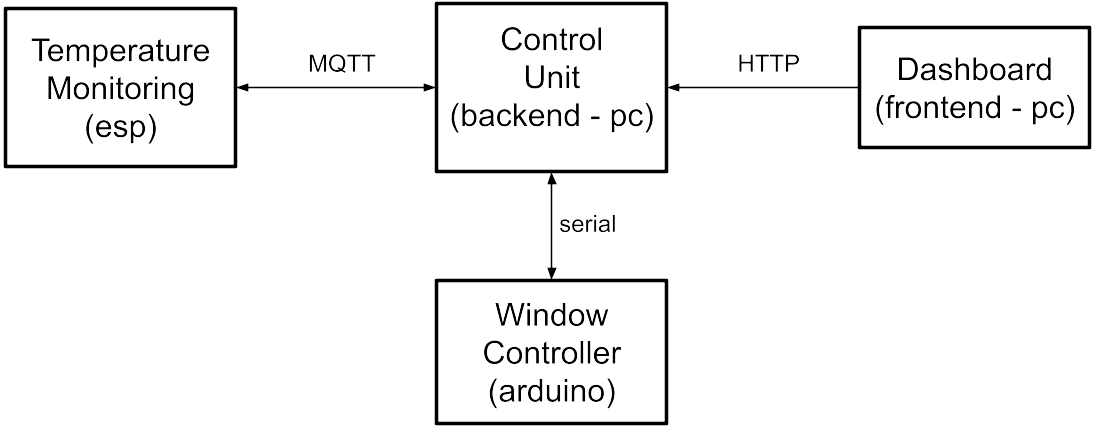
\includegraphics[width=350pt]{report/img/Assignment-03_SMT-Domain.png}
            \caption{Smart Temperature Monitoring}
            \label{img:system}
        \end{figure}


    \section{Requirements}

        \begin{itemize}
            \item The control unit and the temperature sensor have to communicate via the mqtt protocol.
            \item The control unit, the window, and its user panel have to communicate via serial line.
            \item The control unit and the dashboard have to communicate via the http protocol.
            \item The control unit stores the current data of the entire system and tracks the temperature by storing the last $N$ measurements, the maximum, the minimum and the average sampled.
            \item The temperature sensor must sample and send to the control unit the temperature at a frequency established by the control unit based on the current temperature state (\textit{NORMAL, HOT, TOO\_HOT, ALARM}).
            \item The temperature state is established by the temperature and duration of it.
            \item The window opening is decided by the control unit when the window is in \textit{AUTOMATIC MODE}. It depends by the temperature state and the temperature itself.
            \item The window opening when the window is in \textit{MANUAL MODE} is set manually by the user through the user panel, or by an operator through the dashboard.
            \item The window mode can be switched by pressing a button in the user panel or in the dashboard.
            \item The dashboard displays the data stored by the control unit, in particular the temperature history is displayed in a chart.
            \item When the temperature is too high for too long the system goes in \textit{ALARM} state. To return in \textit{NORMAL} state occurs an operator fixing the issue from the dashboard.
        \end{itemize}

\end{document}
